%----------------------------------------------------------------------------------------
%	1. Backgrounds
%----------------------------------------------------------------------------------------

Expert knowledge lies at the core of a medical intelligence system. For example, a doctor would know the proper questions to ask a patient if they want to diagnose a rheumatoid arthritis instead of a simple joint injury. This is also what we expect a medical question answering system would be able to do. A common way to equip machines with knowledge is through a knowledge graph composed of concepts and relations. As the opening part of this tutorial, this section introduces fundamental infrastructures in biomedical informatics, i.e., medical concepts and relations between them, along with the available resources.


\subsection{Concepts and Relations}
\label{sec:1.1}
% what is a concept and what is a relation
For beginners in biomedical informatics, it is important to figure out the meaning of \emph{concept} and \emph{relation}. 
Let's look at an example in our daily life. One day one of your friend feels ill and goes to see a doctor. They say \emph{I have a stomachache! It's killing me!} Then, the doctor tries to comfort them by saying \emph{Your stomach pain will be okay. It looks like a minor stomach disorder.} In this case, we got three medical terms: \emph{stomachache}, \emph{stomach pain}, and \emph{stomach disorder}. Moreover, we can find some connections between these terms:

\begin{enumerate}
  \item The terms \emph{stomachache} and \emph{stomach pain} refer to the same syndrome (or concept).
  \item The disease \emph{stomach disorder} may cause \emph{stomachache}.
\end{enumerate}

First, it is obvious that \emph{stomachache} and \emph{stomach pain} refer to the same \textbf{concept}. Furthermore, with the exception of disease and symptom, every abstract medical entity can be regarded as a concept. They can be procedures, medicine, disorders, mental condition, etc.

Second, there is a \textbf{relation} called \emph{may\_cause} between \emph{stomach disorder} and \emph{stomachache}. This enables the doctor to make a diagnosis for your friend according to their symptoms and the relation between symptoms and diseases. Besides, there are a lot of other relations between concepts. For instance, Aspirin could relieve physical pain; Hypertensive disease may cause heart failure. These relations are crucial to biomedical informatics because they can reveal to us how medical concepts interact with each other. 


\subsection{The necessity of a unified coding system}
In Section \ref{sec:1.1}, we take an example from our daily life to help you understand the meaning of concept and relation. However, biomedical informaticsas an exclusively practical subject, derives its resources from various sources, including but not restricted to textbooks, Wikipedia, and electronic health records (EHR). There are thus great challenges to extracting concepts and relations from the resources, as they not only vary in text style and quality, but also in formats and structures. Therefore, we need a giant \textbf{dictionary} to help us deal with these problems.

In the example from the last section, it is obvious that \emph{stomachache} and \emph{stomach pain} refer to a same concept. However, if a researcher is dealing with EHRs from 10,000 patients, finding out all the mentions of the same concept will be arduous work because doctors may use various terms to refer to the same disease in their records such as \emph{type 2 diabetes}, \emph{adult-onset diabetes}, and \emph{diabetes mellitus type 2}. Nonetheless, if you have a \textbf{dictionary} containing all terms under the same concept, you can find all these mentions easily by direct matching.

Moreover, in the last section, we mentioned that doctors can make diagnoses according to relations between symptoms and diseases. Similarly, If we can gather large quantities of relations between medical concepts, it will be a great help to many fields of biomedical informatics such as auto-diagnosis and relation extraction. Therefore, we hope the \textbf{dictionary} also contains the relations between its concepts.

Do we have such a comprehensive dictionary? Of course! In the field of biomedical informatics, we call the giant dictionary \textbf{a unified coding system}. 


\subsection{UMLS: Unified Medical Language System}
% 改得简略一些
UMLS (Unified Medical Language System)~\cite{10.1093/nar/gkh061} is a large language system that unifies medical concept coding, typing, relations between medical concepts, etc. It is not only a standard, but also a large database. In brief, the UMLS is a comprehensive dictionary containing considerable medical terms and relations between them. 

You can download data and consult the documentation on the UMLS website \footnote{The website of the UMLS is  \url{https://www.nlm.nih.gov/research/umls/index.html}}. 

\subsubsection{Concepts as CUIs in UMLS}
% introduce the approximate number and categories (disease, lab, etc ?) of concepts covered in UMLS, and how and in which table they are stored
% some of the other important fields in the table (e.g. STR, types)
% 原table 1可以保留,但是要同时给文字说明,着重强调重要的字段
It is desirable to have a unique identifier for each concept. In the UMLS, the identifier is called \textbf{CUI} (Unique Concept Identifier). The CUI consists of a \emph{C} followed by several digits such as C0021400 (Influenza). 

As we mentioned in the last section, each concept usually has more than one name or aliases. In the UMLS, we refer to these names or aliases as \textbf{String}. Thus, we can say that each CUI usually has more than one string. 

Among all strings under the same concept, there is always a \textbf{preferred} string which is seen as a preferred name of the concept. Researchers usually use preferred names to refer to Concepts because CUIs are difficult to recognize by humans. 

All of the CUIs and strings are defined by table \textbf{MRCONSO} in the UMLS which contains 4,536,653 concepts with 16,543,671 strings in total. Table~\ref{tab:Identifiers in UMLS} is an example of a concept with its strings.

\begin{table}[ht]
\centering

\begin{threeparttable}[b]
    % part1: setting
    \caption{An example of CUIs and strings in UMLS}
    \label{tab:Identifiers in UMLS}
    
    % part2: tabular
    \begin{tabular}{ccc}
    \toprule
    \textbf{Concept (CUI)}             & \textbf{Preferred string of concept}            & \textbf{All strings of concept}\tnote{1} \\ \midrule
    \multirow{4}{*}{\textbf{C0004238}} & \multirow{4}{*}{\textbf{Atrial Fibrillation}} & Atrial Fibrillation         \\ 
     &  & Atrial Fibrillations    \\  
     &  & Auricular Fibrillation  \\ 
     &  & Auricular Fibrillations \\ 
    \bottomrule
    \end{tabular}
    
    % part3: notes
    \begin{tablenotes}
    \item [1] Usually, there are some duplicate strings under the same CUI. Make sure you remove the duplication when constructing your own dictionary. 
    \end{tablenotes}

\end{threeparttable}

\end{table}


In addition to CUIs and strings, MRCONSO also provides other information about medical terms, such as language, source vocabularies, types, etc. The MRCONSO is a table of the UMLS, and here~\footnote{\url{https://www.ncbi.nlm.nih.gov/books/NBK9685/table/ch03.T.concept_names_and_sources_file_mr/}} is the description of all columns of the table. Here, we only introduce some of them:

\begin{enumerate}
  \item \textbf{CUI}: Unique identifier for concept
  \item \textbf{LAT}: Language of the term
  \item \textbf{STR}: String of the term
  \item \textbf{SUPPRESS}: Suppressible flag, indicating whether the entry is obsolete
\end{enumerate}

With the entries in MRCONSO, we can extract all strings under the same CUI easily. \par

\subsubsection{Different versions of CUIs}
Over time, CUIs get retired or merged with other CUIs. This happens when
\begin{enumerate}
\item Two released concepts are found to be synonyms so only one is kept 
\item The concept is not present in any of the current source vocabularies
\item The concept is an acknowledged error in a source vocabulary or determined to be a Metathesaurus production error.
\end{enumerate}

This information can be tracked using the \textbf{MRCUI} table

\subsubsection{Relations in UMLS}
Relations between concepts in the UMLS are defined in another table called \textbf{MRREL}. Each entry of this table provides a relation between a pair of concepts. Let's look at the example in table~\ref{tab:relations example}. \par

\begin{table}[ht]
\centering
\caption{An example of relations in UMLS}
\label{tab:relations example}
\begin{tabular}{ccccc}
\toprule
\textbf{CUI1} & \textbf{REL} & \textbf{CUI2} & \textbf{RELA}          & \textbf{SUPPRESS} \\ \midrule
C4707509      & RO           & C0004057      & active\_ingredient\_of & O                 \\ \bottomrule
\end{tabular}
\end{table}

Table~\ref{tab:relations example} presents an entry extracted from the table MRREL (some columns are omitted), which means that \emph{C0004057 (Aspirin)} is the active ingredient of \emph{C4707509 (Aspirin 800mg gastro-resistant oral tablet)}. However, the attribute \emph{SUPPRESS} is \emph{O}, which means that the entry is probably obsolete. Usually, we only use entries with  \emph{SUPPRESS} = \emph{N}. \par

The official document~\footnote{\url{https://www.ncbi.nlm.nih.gov/books/NBK9685/table/ch03.T.related_concepts_file_mrrel_rrf/}} provides the description of all of the columns in MRREL. We only introduce some of them here: \par
\begin{enumerate}
  \item \textbf{CUI1/AUI1}: Unique identifier of first concept/atom
  \item \textbf{CUI2/AUI2}: Unique identifier of second concept/atom
  \item \textbf{REL}: Relationship of second concept or atom to first concept or atom
  \item \textbf{RELA}: Additional (more specific) relationship label
  \item \textbf{SUPPRESS}: Suppressible flag, indicating whether the entry is obsolete
\end{enumerate}

The column \textbf{RELA} is more frequently used than \textbf{REL} because RELA provides much more specific information than REL does. REL only has 13 kinds of sketchy relations such as \emph{has a narrower relationship} and \emph{related and possibly synonymous}. On the other hand, RELA provides hundreds of relations such as \emph{induces},  \emph{ingredient\_of} and \emph{isa}(is a).


\subsection{Semantic Types in UMLS}
In the previous section, We discussed concepts (CUIs) and relations provided by the UMLS. 
The UMLS also provides categories of these concepts and relations between these categories. 
These categories are called \textbf{Semantic Types} and the relations are called \textbf{Semantic Relations}.
They constitute the \textbf{Semantic Network} of the UMLS.
The Semantic Network contains 127 semantic types and 54 relationships.
Each concept (CUI) may have more than one semantic type.

\begin{table}[ht]
\centering
\caption{Hierarchy of Semantic Types}
\label{tab:semantic hierachy}

\begin{tabular}{@{}cll@{}}
\toprule
\multicolumn{1}{l}{Level 1} & Level 2                              & Level 3                       \\ \midrule
\multirow{5}{*}{Biologic Function} & \multirow{2}{*}{Physiologic Function} & Disease or Syndrome \\
                            &                                      & Experimental Model of Disease \\ \cmidrule(l){2-3} 
                            & \multirow{3}{*}{Pathologic Function} & Cell Function                 \\
                            &                                      & Molecular Function            \\
                            &                                      & Organism Function             \\ \bottomrule
\end{tabular}

\end{table}

Table~\ref{tab:semantic hierachy} illustrates the Hierarchy of Semantic Types. The semantic type "Biologic Function" has two children, "Physiologic Function" and "Pathologic Function", and each of these in turn has several children, too. 
Each child in the hierarchy is linked to its parent by the "isa" link.

The relations between Semantic Types are also hierarchical.
They are grouped into five major categories, which are themselves relations: "physically related to", "spatially related to", "temporally related to", "functionally related to", and "conceptually related to".

\subsubsection{Accessing the UMLS}
Since the UMLS is a typical relational database, it is convenient to access its tables with any programming language such as Python, Java, R, etc. 
You can consult the official document of Metathesaurus\footnote{\url{https://www.ncbi.nlm.nih.gov/books/NBK9685/}} and Semantic Networks\footnote{\url{https://www.ncbi.nlm.nih.gov/books/NBK9679/}} to know about the structures of tables and files.
Here we provide some demos for accessing UMLS in Python. The package \emph{Pandas} is needed.

Access and clean the MRCONSO.RRF (it defines all CUIs in the UMLS) in Metathesaurus:
\begin{python}
import pandas as pd

MRCONSO_PATH = '2021new/MRCONSO.RRF'

# columns of MRCONSO
column_conso = ['CUI','LAT','TS','LUI','STT','SUI','ISPREF','AUI',
'SAUI','SCUI','SDUI','SAB','TTY','CODE','STR','SRL','SUPPRESS','CVF']

# read MRCONSO
conso = pd.read_csv(MRCONSO_PATH, dtype='str', sep='|', 
        names=column_conso, usecols=column_conso, index_col=False)
print('mrconso size:', conso.shape)

# delete non-English and empty words
conso = conso[(conso['LAT'] == 'ENG') & (~conso['STR'].isna())]
    
# delete obsolete words
conso = conso[conso['SUPPRESS'] == 'N']

# ......
# ......
# you can do further cleaning with more operations
\end{python}

Access the MRSTY.RRF (it provides Semantic Type assigned to each concept) in Metathesaurus:
\begin{python}
'''
Code above that loads MRCONSO
'''

MRSTY_PATH = '2021new/MRSTY.RRF'

# columns of MRSTY
column_sty = ['CUI', 'TUI', 'STN', 'STY', 'ATUI', 'CVF']

# read MRSTY
sty = pd.read_csv(MRSTY, dtype='str', sep='|', names=column_sty, 
        usecols=column_sty, index_col=False)
print('mrsty size:', sty.shape)

# keep all entries with CUI in the cleaned MRCONSO
all_cui = set(conso['CUI'])
sty = sty[sty['CUI'].isin(all_cui)]
print('final sty', sty.shape)
\end{python}

\subsection{Concepts as codes in other coding systems}
Apart from CUIs in the UMLS, there are other common coding systems and they each will be introduced in this section. Most of them are specialized coding systems that encode a specific type of concept including diseases, medications, procedures and laboratory codes.
\subsubsection{Disease codes}
Disease codes encode certain diseases, symptoms, and phenotypes into a unique code. Typical disease coding systems include ICD (International Classification of Diseases) codes\footnote{\url{https://www.who.int/standards/classifications/classification-of-diseases}}, Phecodes\footnote{\url{https://phewascatalog.org/phecodes}}, and HPO (Human Phenotype Ontology) codes\footnote{\url{https://hpo.jax.org/app/}}. People from different countries or different hospitals may use different coding systems for applications includingEHR and insurance.

\textbf{ICD Codes}

The International Classification of Diseases Codes (ICD) is a list of codes for diseases, symptoms, findings, and injuries that is maintained by the World Health Organization (WHO). ICD codes are used to record medical findings in a standardized format in EHR and to track global morbidity and mortality data. Different countries and different hospitals may use different versions of ICD codes. WHO periodically releases new versions of ICD codes, among which ICD-9 and ICD-10 are relevant to EHR data. The United States uses an extended version of ICD called the "clinical modification" (CM), e.g. ICD-9-CM. ICD-10-CM has over five times the number of diagnosis codes as ICD-9-CM.

\textbf{Phecodes}

Closely related to the ICD codes, Phecodes are phenotyping codes that group various ICD codes into useful phenotypes. ICD codes are very detailed codes, which can be manually rolled up to phecodes \cite{icd9-phecode,icd10-phecode}. Phecodes version 1.2 condenses roughly 15500 ICD-9-CM codes and 90000 ICD-10-CM codes into 1867 phecodes. ICD codes and phecodes create a certain hierarchy\footnote{The figure is obtained from a visualization tool for ICD codes and phecodes.  \url{https://hmsrsc.aws.hms.harvard.edu/content/89/}} from general phenotype to detailed findings. An example of this hierarchy is shown in Figure \ref{fig:phecode_hier}.A complete ICD-Phecodes system includes ICD codes, ICD strings, corresponding phecodes and phenotypes, and corresponding excluded phecodes range and phenotype. Table \ref{phecode} shows an example of the ICD-Phecodes system. 
\begin{figure}[ht]
    \centering
    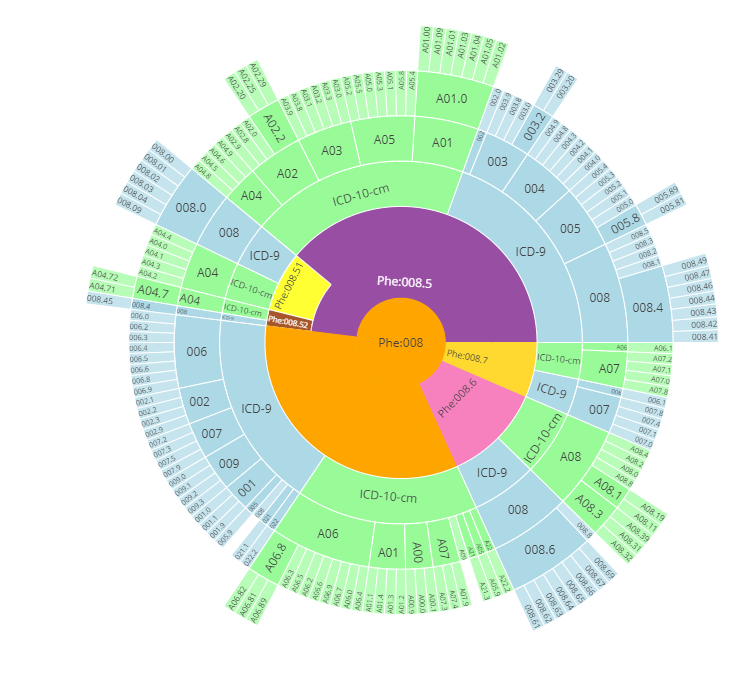
\includegraphics[width=0.9\linewidth]{images/phecode_hierarchy.png}
    \caption{An example of the ICD-Phecode hierarchy. The most general concept (root) is encoded as an integer in the phecode system, e.g. 008. The second level is encoded as a decimal with the same integer part as the root and one digit after the decimal point, while the third level has two digits after the decimal point. Each phecode groups a part of ICD codes.}
    \label{fig:phecode_hier}
\end{figure}

\begin{table}[ht]
\centering

\resizebox{\linewidth}{!}{%
\begin{tabular}{llllll}
\toprule
ICD-9  & ICD-9 String                                                                  & Phecode & Phenotype                         & Excl. Phecodes & Excl. Phenotypes \\ \hline
250    & Diabetes mellitus                                                             & 250     & Diabetes mellitus                 & 249-250.99       & DIABETES           \\
250.1  & Diabetes with ketoacidosis                                                    & 250     & Diabetes mellitus                 & 249-250.99       & DIABETES           \\
250.33 & Diabetes mellitus with other coma...   & 250.1   & Type 1 diabetes                   & 249-250.99       & DIABETES           \\
250.13 & type I diabetes mellitus {[}juvenile type{]}... & 250.11  & Type 1 diabetes with ketoacidosis & 249-250.99       & DIABETES     \\
\bottomrule
\end{tabular}%
}
\caption{An example of ICD-Phecode system. ICD codes are grouped by phecodes and phenotypes. Numbers after the decimal point of phecodes show certain hierarchies of phenotypes. For example, 250---250.1---250.11 represents the hierarchy of Diabetes mellitus---Type 1 diabetes---Type 1 diabetes with ketoacidosis.}
\label{phecode}
\end{table}
% Phecodes are created by Clinical Classification Software (CCS) grouping schema. 

\textbf{HPO Codes}

The Human Phenotype Ontology (HPO) provides a standardized vocabulary of phenotypic abnormalities encountered in human disease. HPO mainly consists of two parts; ontology and annotations. The ontology contains detailed information of each term, including id, name, definition, and basic properties such as synonyms, "is-a" relations and cross references. Annotations contain phenotype annotations for certain diseases (whether and how certain diseases will show certain phenotypes or features). They are linked with databases like OMIM \cite{omim} or DECIPHER \cite{decipher}. In the annotation file, each line represents a link between a disease entity such as \textit{Noonan syndrome} and one of the clinical features characteristically seen in that disease. Examples of the ontology system and annonations are shown in Figure \ref{fig:hpo_annotate_example}

HPO currently contains over 13,000 terms and over 156,000 annotations to hereditary diseases. Its detailed descriptions of clinical abnormalities and computable disease definitions have made it the standard for deep phenotyping in the field of rare diseases \cite{hpo}. HPO can also be mapped to other coding systems like phecodes \cite{hpo,hpo-phecode}.
\begin{figure}[ht]
    \centering
    \begin{subfigure}[b]{0.9\textwidth}
      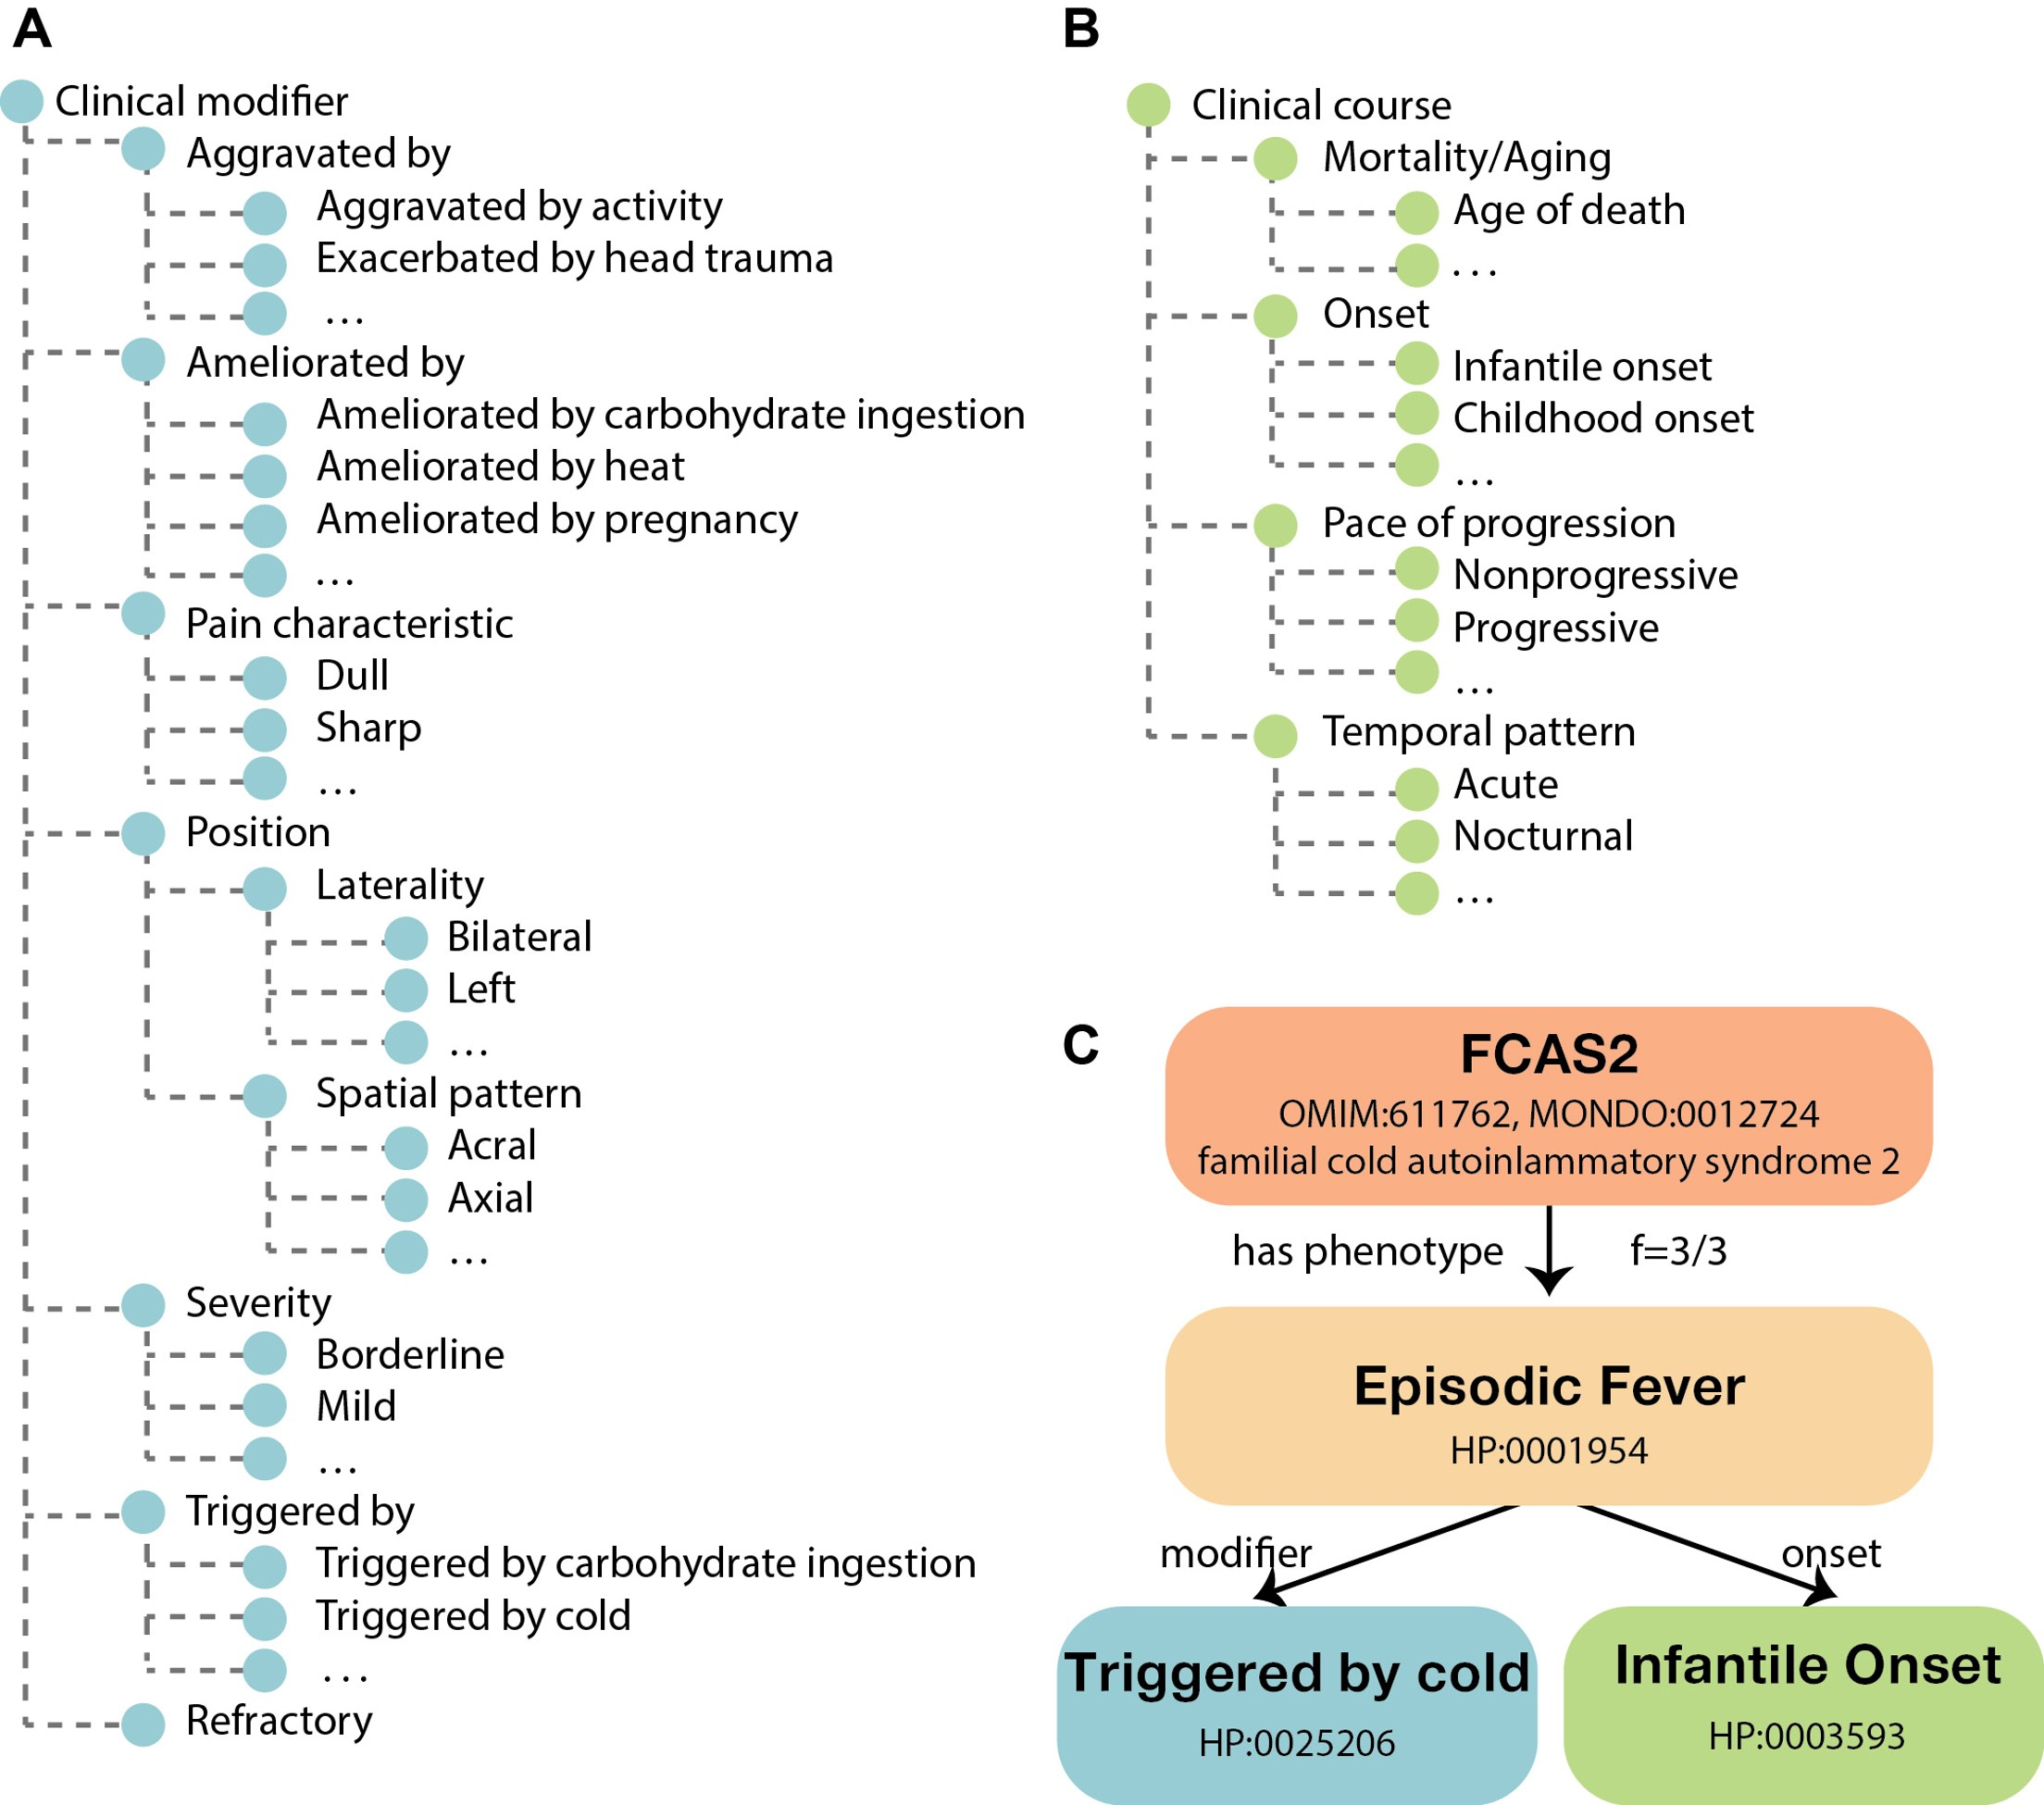
\includegraphics[width=\linewidth]{images/hpo annotation example.jpg}
    \end{subfigure}
    \begin{subfigure}[b]{0.9\textwidth}
      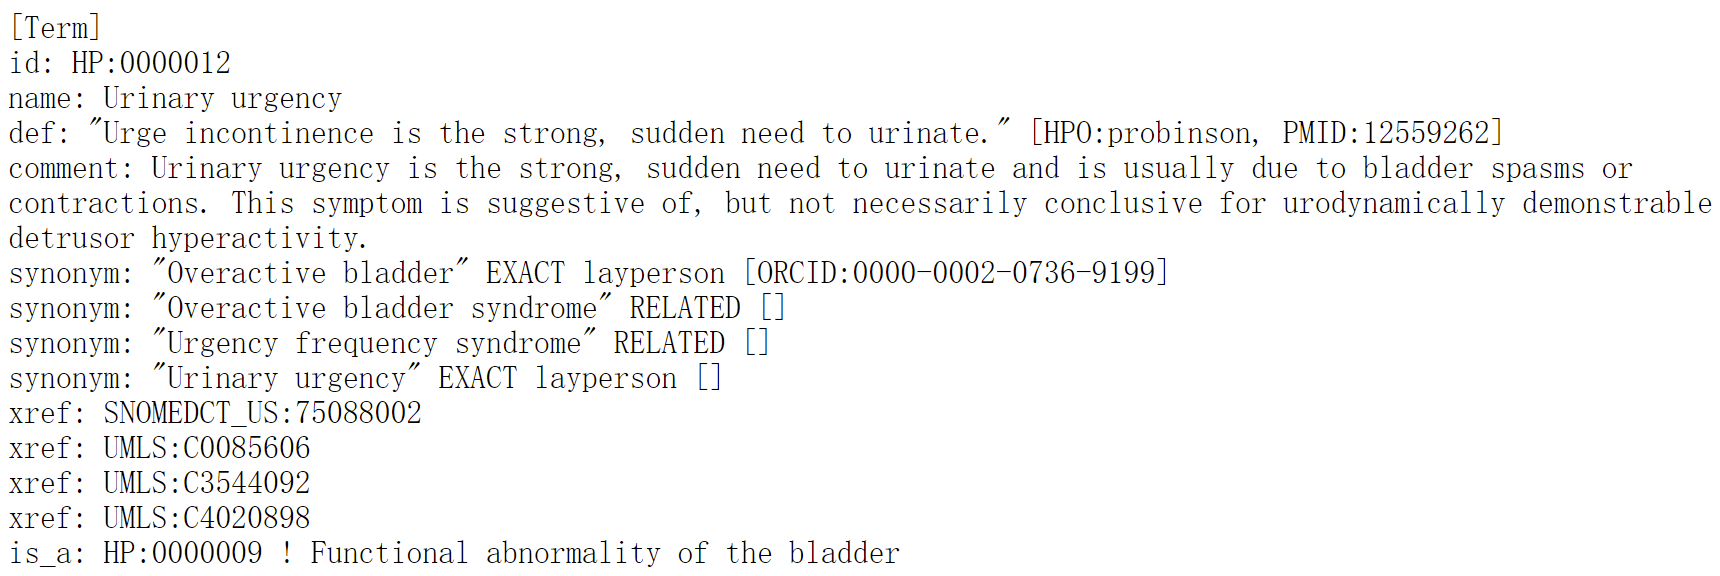
\includegraphics[width=\linewidth]{images/hpo ontology.png}
    \end{subfigure}    
    \caption{\textbf{UP}: An example of HPO annotations for familial autoinflammatory syndrome 2 introduced by \cite{hpo}. As is shown in (C), one annotation mainly consists of a disease, a phenotype, and its clinical modifiers and courses (sub-ontologies). This example demonstrates that, in a publication on this disease, three of three reported patients were found to have episodic fever with infantile (or earlier) onset that was triggered by exposure to cold. General format of annotations is described in \cite{hpo} and \url{https://hpo.jax.org/app/help/annotations}. \textbf{DOWN}: An example of HPO ontology in OBO flat file format obtained from \href{https://raw.githubusercontent.com/obophenotype/human-phenotype-ontology/master/hp.obo}{hp.obo} which shows the properties of phenotype "Urinary urgency". OWL version of the HPO which contains more definitions like logical difinitions can be found in \url{https://hpo.jax.org/app/download/ontology}.}
    \label{fig:hpo_annotate_example}
\end{figure}


\subsubsection{Medication codes}
Medication codes encode drug products and their usage into unique codes. Typical medication coding systems include RxNorm\footnote{https://www.nlm.nih.gov/research/umls/rxnorm/index.html} and National Drug Code (NDC)\footnote{https://www.fda.gov/drugs/drug-approvals-and-databases/national-drug-code-directory}. Medication codes are used in billing or EHR.

\textbf{RxNorm}

RxNorm, produced by The National Library of Medicine (NLM), provides normalized names for clinical drugs and links its names to many of the drug vocabularies commonly used in pharmacy management and drug interaction software, including those of First Databank, Micromedex, and Gold Standard Drug Database. RxNorm provides a set of codes (RxCUI) for clinical drugs, which are the combination of active ingredients, dose form, and strength of a drug. For example, the RxCUI for \textit{ciprofloxacin 500 mg 24-hour extended-release tablet} (the generic name for Cipro XR 500 mg) is RX10359383, regardless of brand or packaging. RxNorm is also a hierarchical code, with relationships like "has\_precise\_ingredient", "has\_ingredient", "has\_part", and "consists\_of". 

RxNorm can be downloaded directly through \url{https://www.nlm.nih.gov/research/umls/rxnorm/docs/rxnormfiles.html}. The RRF files of RxNorm are just like those of UMLS. The file types are listed in Table \ref{tab:rxnormtype} and their formats are presented in \href{https://www.nlm.nih.gov/research/umls/rxnorm/docs/techdoc.html#s12_0}{RxNorm Technical Documentation}. RxNorm can be also navigated through \href{https://mor.nlm.nih.gov/RxNav/}{RxNav}, which offers a visualized browser for each RxNorm code. Examples of RxNav is shown in Figure \ref{fig:rxnav}.

\begin{figure}[ht]
    \centering
    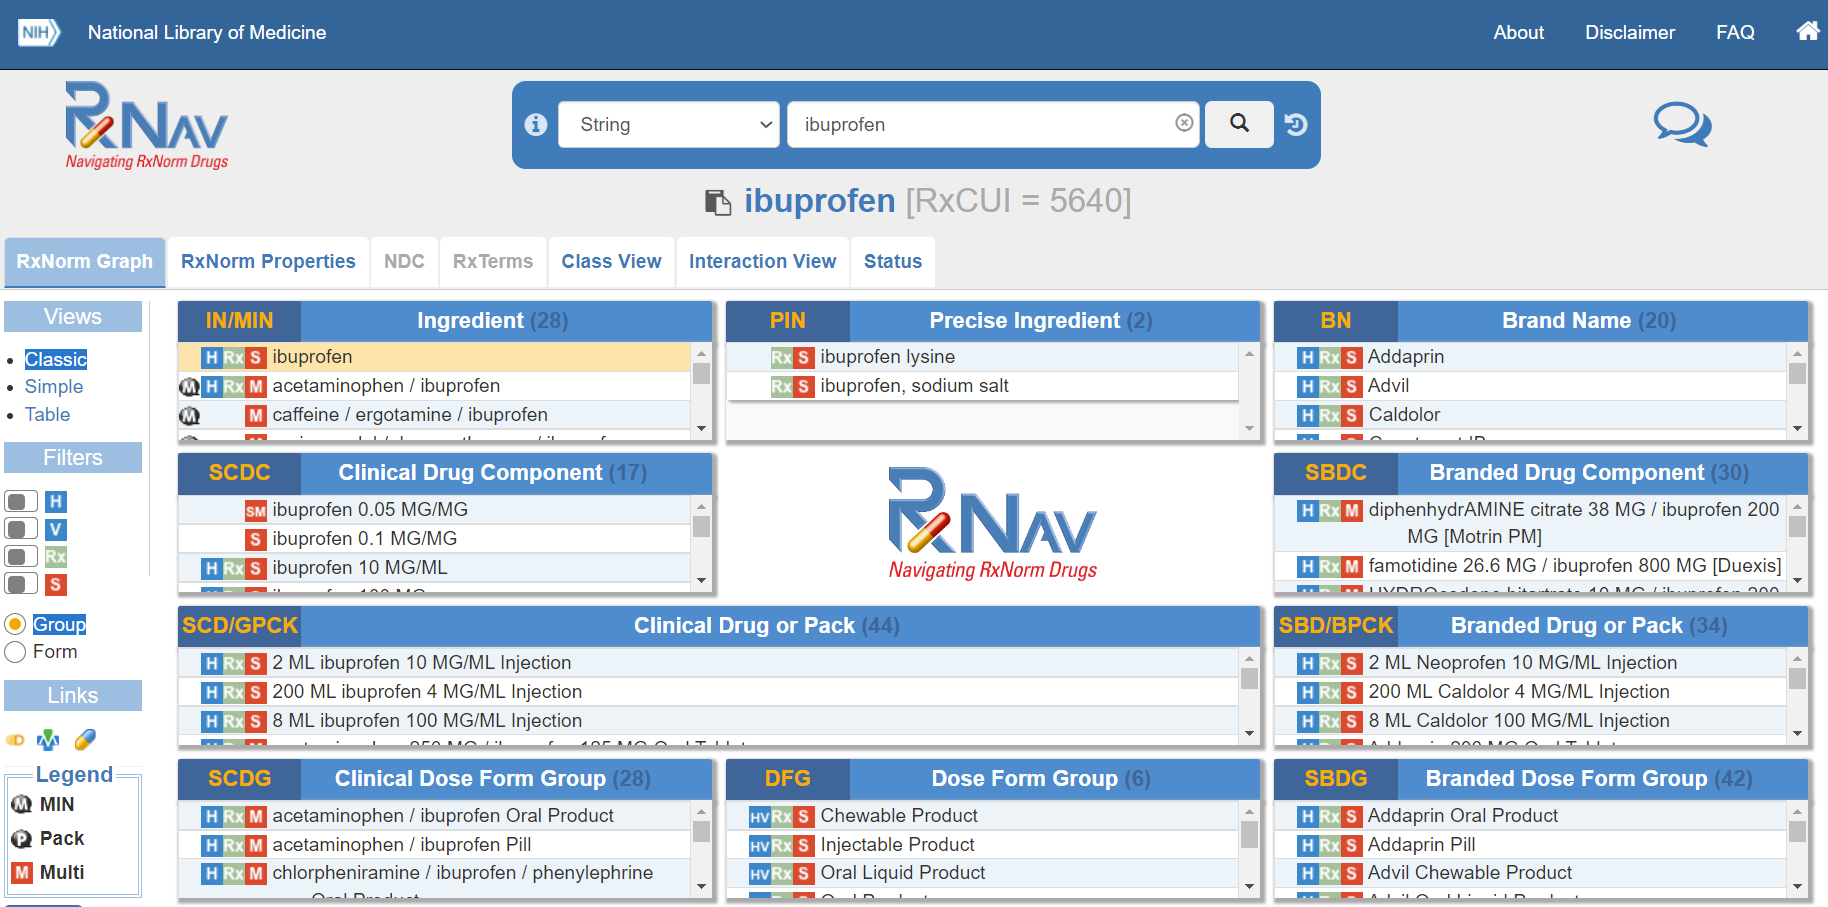
\includegraphics[width=0.9\linewidth]{images/rxnav.png}
    \caption{An example of RxNav for Ibuprofen. The browser shows properties like ingredients and clinical drug components of Ibuprofen. RxNav provides an interactive tool for RxNorm.}
    \label{fig:rxnav}
\end{figure}

\begin{table}[ht]
\centering
\begin{tabular}{ll}
\toprule
Concepts, Concept Names, and their sources & RXNCONSO.RRF                       \\ 
Attributes                                 & RXNSAT.RRF, RXNSTY.RRF             \\ 
Relationships                              & RXNREL.RRF                         \\ 
Data about RxNorm                          & RXNDOC.RRF, RXNSAB.RRF, RXNCUI.RRF \\ 
Archive Data                               & RXNATOMARCHIVE.RRF                 \\ 
Concept Changes Tracking Data              & RXNCUICHANGES.RRF                  \\ \bottomrule
\end{tabular}
\caption{File types of RxNorm.}
\label{tab:rxnormtype}
\end{table}

\textbf{NDC}

The National Drug Code (NDC) is a unique product identifier used in the United States for drugs intended for human use. It's published by U.S. Food and Drug Administration (FDA). Through NDC, drugs are identified and reported using a unique, three-segment number which serves as the FDA's identifier for drugs. 

The first segment, the labeler code, is 4, 5 or 6 digits long and identifies the labeler such as the drug manufacturer, repackager, or distributer. The second segment, the product code, is 3 or 4 digits long and identifies a specific strength, dosage form, and formulation for a particular firm. The third segment, the package code, is 1 or 2 digits long and identifies package forms and sizes. For example, the product NDC of \textit{Ibuprofen} produced by Granules India Limited is 62207-0356.

\subsubsection{Procedure codes}
Procedure codes are a sub-type of medical classification used to identify specific surgical, medical, or diagnostic procedures. Typical procedure codes include Current Procedural Terminology (CPT) and ICD-10 Procedure Coding System (ICD-10-PCS). Procedure codes are used in billing, EHR, and insurance.

\textbf{CPT}

The Current Procedural Terminology (CPT) code set is a procedural code set developed by the American Medical Association (AMA). The CPT code set describes medical, surgical, and diagnostic procedures for administrative, financial, and analytical purposes. There are three types of CPT codes. Category 1 are 5-digit codes that cover evaluation and management, anesthesiology, surgery, radiology, pathology and laboratory, and medicine. These are the most widely used CPT codes. Category 2 are clinical laboratory services and category 3 are emerging technologies, services and procedures. Examples of CPT codes are listed in Table \ref{tab:cpt}.

\begin{table}[ht]
\centering
\begin{tabular}{ll}
\toprule
CPT & Name \\ \hline
3120F & 12-LEAD ECG PERFORMED               \\ \hline
4030F & LONG-TERM OXYGEN THERAPY PRESCRIBED \\ \hline
0575F & HIV RNA CONTROL PLAN OF CARE DOCD   \\ \bottomrule
\end{tabular}
\caption{Examples of CPT codes.}
\label{tab:cpt}
\end{table}

\textbf{ICD-10-PCS}

The ICD-10 Procedure Coding System (ICD-10-PCS) is an international system of medical classification used for procedural coding. ICD-9-CM contains a procedure classification while ICD-10-CM does not, so ICD-10-PCS is the procedure classification for ICD-10. Each ICD-10-PCS code consists of seven alphanumeric characters. The first character is the 'section'. The second through seventh characters mean different things in each section. Each character can be any of 34 possible values the ten digits 0-9 and the 24 letters A-H, J-N and P-Z may be used in each character. The letters O and I are excluded to avoid confusion with the numbers 0 and 1. There are no decimals in ICD-10-PCS. Of the 72,081 codes in ICD-10-PCS, 62,022 are in the first section, "Medical and surgical". Detailed descriptions of the sections can be found in \href{https://en.wikipedia.org/wiki/ICD-10_Procedure_Coding_System#Section_structure}{Wiki}. For example, 07Q70ZZ is the code for \textit{Repair Thorax Lymphatic, Open Approach}.

\subsubsection{Laboratory codes}
Laboratory codes identify medical laboratory observations. The Logical Observation Identifier Names and Codes (LOINC) is the most widely-used laboratory codes.

\textbf{LOINC}

The Logical Observation Identifier Names and Codes (LOINC) database provides a universal code system for reporting laboratory and other clinical observations. The database currently has over 71,000 observation terms. A LOINC term includes 6 parts: component, kind of property, time aspect, system, type of scale, and type of method. An example of LOINC term is shown in Table \ref{tab:Example of clinical LOINC terms and names }.

LOINC has a hierarchical structure. It can be represented as a tree, where each leaf is the LOINC term and the parents are LOINC parts (whose codes are started with LP, e.g. LP14559-6 stands for \textit{Bacteria}). A visualization of such structure can be browsed in \url{https://loinc.org/tree/}. 

% Its purpose is to identify observations in electronic messages such as Health Level Seven (HL7) observation messages, so that when hospitals, health maintenance organizations, pharmaceutical manufacturers, researchers, and public health departments receive such messages from multiple sources, they can automatically file the results in the right slots of their medical records,research, and/or public health systems.

% The main categories of laboratory test procedures that are included in the LOINC database are identified in Table~\ref{tab:Laboratory LOINC scope} along with the number of LOINC terms defined for each category.


% \begin{table}[ht]
% \centering
% \caption{Laboratory LOINC scope
% }
% \label{tab:Laboratory LOINC scope}
% \begin{tabular}{|c|c|c|c|}
% \hline
% \textbf{Class} & 
% \textbf{No. of terms} & 
% \textbf{Class} & 
% \textbf{No. of terms}\\ \hline
% Antibiotic susceptibilities  & 
% 	1010 & 
% Hematology cell count & 
% 1082  
% \\ \hline

% Blood bank   & 
% 		658 & 
% 	Microbiology  & 
% 5786
% \\ \hline

% Chemistry    & 
% 		4817  & 
% Molecular pathology  & 
% 245 
% \\ \hline

% Coagulation    & 
% 	346  & 
% 	Skin tests   & 
% 25 
% \\ \hline

% Cytology     & 
% 	31   & 
% Pathology   & 
% 	124 
% \\ \hline

% Fertility     & 
% 	123   & 
% Drug and toxicology   & 
% 3919 
% \\ \hline

% Flow cytometry cell markers     & 580    & 
% Urinalysis    & 
% 136 
% \\ \hline
% \end{tabular}
% \end{table}
% \textbf{Examples}

% The LOINC clinical observation name (which includes laboratory test results, clinical measurements, and other diagnostic studies) must include six main items:
% \begin{enumerate}
%   \item \textbf{Component (analyte)}: e.g., potassium, hemoglobin, hepatitis B antigen
%   \item \textbf{Property measured}:e.g., a mass concentration, enzyme activity (catalytic rate)
%   \item \textbf{Timing}:i.e., whether the observation applies to a moment in time or is an average or amount taken over a period of time, as is the case for a 24-h urine sodium concentration 
%   \item \textbf{System}:i.e., type of sample or organ examined: e.g., urine, blood, chest
%   \item \textbf{Scale}:e.g., whether the measurement is quantitative (a true measurement), ordinal (a ranked set of options), nominal, or narrative (e.g., dictation results from x-rays)
%   \item \textbf{Method}:Method used to produce the observation, but only when different methods give clinically significant different results
% \end{enumerate}

% An example of clinical LOINC terms and names is shown in Table~\ref{tab:Example of clinical LOINC terms and names }. , in which each of the items is separated into a separate column for easier reading.The Loinc code 29463-7 represents Body weight. Its attribute type is Mass, its time feature is point in time, its system is \^\ Patient, and its scale is quantitative.

\begin{table}[ht]
\centering

\begin{tabular}{|c|c|c|c|c|c|c|}
\hline
\textbf{Code} & 
\textbf{Component} & 
\textbf{Property} & 
\textbf{Time aspect}&
\textbf{System}&
\textbf{Scale}&
\textbf{Method}\\ \hline
29463-7 & 
Body weight & 
Mass & 
Pt &
\^\ Patient &
Qn &
---
\\ \hline
\end{tabular}
\caption{Example of LOINC term \textit{body weight}. Component indicates what is measured, evaluated, or observed. Property indicates characteristics of what is measured. Time aspect indicates interval of time over which the observation or measurement was made. Pt means point in time. System indicates context or specimen type within which the observation was made, e.g. blood or urine. Scale indicates the scale of measure. Qn means quantitative. Method indicates the procedure used to make the measurement or observation.
}
\label{tab:Example of clinical LOINC terms and names }
\end{table}

% \subsubsection{RxNorm}
% RxNorm is a second vocabulary for prescription drugs. RxNorm provides a set of codes for clinical drugs, which are the combination of active ingredients, dose form, and strength of a drug. For example, the RxNorm code for ciprofloxacin 500 mg 24-hour extended-release tablet (the generic name for Cipro XR 500 mg) is RX10359383, regardless of brand or packaging.Its main uses are as follows:


% 1) Capturing drug information in electronic health record systems using the RxNorm standard name and code. For example, Centers for Medicare and Medicaid Services staff generally use the RxNorm as the standard for documenting drugs. 

% 2) RxNorm can be used in Personal Health Record System (PHR) or Electronic Health Record (EHR).For example, doctors can capture patient medication history data through RxNorm in the EHR system; Meanwhile, physicians can use RxNorm to classify EHR drug data.



% \textbf{Example}

% Detailed technical information about RxNorm can be viewed at\footnote{The official website for RxNorm Code is \url{https://www.nlm.nih.gov/research/umls/rxnorm}.}.After receiving the drug information, NLM outputs this source data in a standard data format to an RxNorm file and groups it into a collection of synonyms called "concepts." Each concept is assigned an RxNorm concept unique identifier (RXCUI), but RXCUI has no inherent meaning. Each concept also has an RxNorm normalized name, which is counted as "SAB = RxNorm". 
% SAB = RXNORM uses different forms of Term types to represent generic and branded drug names, as shown in Table~\ref{tab:RxNorm terminology type format} . 


% The above semantics are related to each other through "relationships", such as "has tradename", "part of", "has dose form", "dose form of", etc., forming the semantic web. Through various terminals of RxNorm, semantic web can retrieve information of other term types of the drug from any form of term types, and realize drug information interaction of different expression levels and the same chemical components through relational transmission. Take Metoprolol tartrate as an example, see Figure ~\ref{fig: Semantic web of metoprolol tartrat} for its semantic web. 
% \begin{table}[ht]
%   \caption{RxNorm terminology type format}
%   \label{tab:RxNorm terminology type format}
%   \centering
%   \begin{tabular}{llll}
%     \toprule
%     Term types     &   Name   &  Describe & Example  \\
%     \midrule
%     IN & ingredient & A compound or ingredient & Metoprolol\\
%     PIN & precision ingredient & An ingredient of a particular form & Metoprolol Tartrate\\
%     BN & brand name & A distinguished family of products name& Lopressor\\
   
%     \bottomrule
%   \end{tabular}
% \end{table}
% \begin{figure}[ht]
% \centering
% 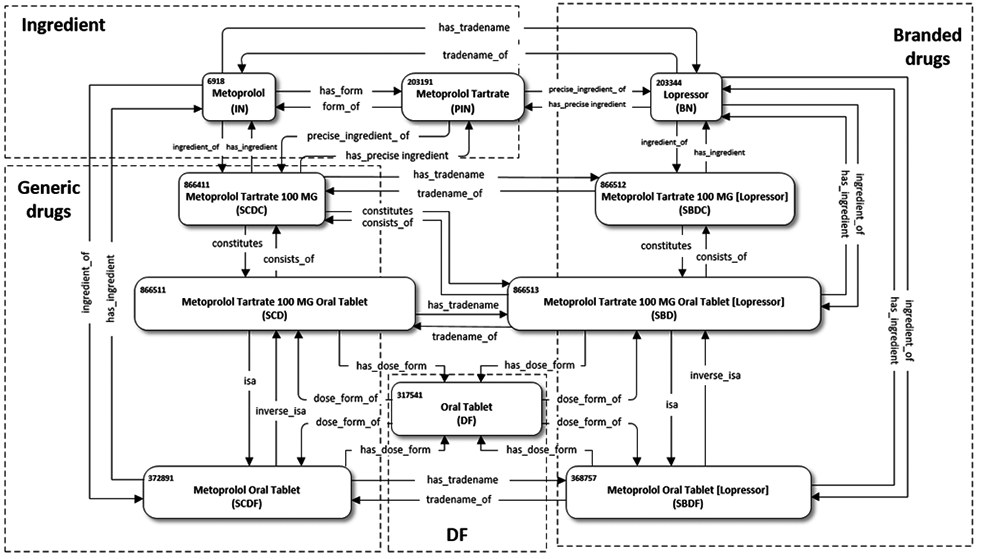
\includegraphics[width=1\textwidth]{images/png1.2.4.png}
% \caption{\label{fig: Semantic web of metoprolol tartrat}Semantic web of metoprolol tartrate.}
% \end{figure}

% \subsubsection{ICD code and Phecode}
% The International Classification of Diseases Codes (ICD) is a list of codes for diseases, symptoms, findings, and injuries that is maintained by the World Health Organization (WHO). ICD codes are used to record medical findings in a standardized format in EHR and track global morbidity and mortality data. WHO periodically releases new versions of ICD codes, among which ICD-9 and ICD-10 are relevant to EHR data. The United States uses an extended version of ICD called the "clinical modification" (CM), e.g. ICD-9-CM. ICD-10-CM has over five times the number of diagnosis codes as ICD-9-CM, which is used until 2015.

% Phecodes are manually curated groups of ICD codes to group various ICD codes into useful phenotypes. Phecodes are created by Clinical Classification Software (CCS) grouping schema. Phecodes are available at \url{https://www.phewascatalog.org/phecodes}. Phecodes version 1.2 condenses roughly 15500 ICD-9-CM codes and 90000 ICD-10-CM codes into 1867 phecodes. Phecodes are also hierarchical, which show the hierarchy between phenotypes through a three-digit parent code and two-digit code following a decimal point. A complete ICD-Phecodes system includes ICD code, ICD string, corresponding phecode and phenotype, and corresponding exclude phecodes range and phenotype. Table \ref{phecode} shows an example of ICD-Phecodes system. 



% \textbf{Importance}

% 1) ICD codes are widely used as a standardized format to record medical findings of patients in EHR in a lot of countries.

% 2) Phecodes is a hierarchical codified system that maps both ICD-9 and ICD-10 codes into one system of phenotypes. Hierarchical information among phenotypes can be obtained from phecodes.

% \textbf{Notes}

% 1) 

% \subsection{CPT and CCS code}

% \subsection{The mapping between systems}
% 现有的一些不同coding system之间的mapping?adding into the subsections



\subsection{Aggregation of codified data} \label{sec:Aggregation of codified data}

EHR data typically include four domains of codified data: diagnosis, procedures, lab measurements, and medications. Due to differential coding practices, the same clinical concepts might be represented by distinct clinical codes at different healthcare systems \cite{hernandez2009automated, abhyankar2012standardizing}. For example, acute myocardial infarction (MI) of anterolateral wall and acute MI of the inferolateral wall are separate codes that describe the same concept of MI \cite{hong2021clinical}. To reduce ambiguity and alleviate  heterogeneity across different healthcare systems, the individual clinical codes are usually rolled to codes representing general concepts \cite{hong2021clinical,zhou2022multiview}. More specifically,  ICD codes are often aggregated into PheCodes using the ICD-to-PheCode mapping from PheWAS catalog (\href{https://phewascatalog.org/phecodes}{https://phewascatalog.org/phecodes}). Procedure codes including CPT-4, HCPCS, ICD-9-PCS, ICD-10-PCS are grouped into clinical classification software (CCS) categories based on the CCS mapping ( \href{https://www.hcup-us.ahrq.gov/toolssoftware/ccs_svcsproc/ccssvcproc.jsp}{https://www.hcup-us.ahrq.gov/toolssoftware/ccs\_svcsproc/ccssvcproc.jsp}). Medication codes are often aggregated and rolled up into ingredient level RxNorm codes. 
Laboratory measurements can be aggregated into LOINC codes and further grouped into higher level LOINC Parts codes (LP codes) to reflect broader laboratory code concepts by leveraging the LOINC Multiaxial Hierarchy \cite{mcdonald2004logical}.













 
 
